\chapter{Theory}
\section{Conversational Analysis}
\subsection{Pause Use}
Pauses are a natural part of any conversation. For a given conversation pauses can express different pieces of information such as confusion, boredom, excitement, reflection, etc \ldots. These pauses can be used to measures specifically what is happening in the conversation at any point in time. However, not all pauses can be thought of as the same. A pause can change significantly in meaning if a receiver pauses for 3s vs 10ms after a speaker utters something (e.g. 3s pause could be attributed to reflection, while 10ms could imply excitement to reply). Analysing how these pauses appear in the conversation can be insightful in understanding specifics about the conversation without requiring semantic level understanding of the speech (e.g. whether the speakers are old or from a different country based on how they use pauses). Pauses themselves can be grouped into types, for example, a pause bookended by the same speaker would be considered an inner pause, while a pause bookended by different speakers would be a joint pause. These pause types can present information such as how the conversations is progressing, who is taking more time speaking, how often a speaker is interrupted, how long silences last for.



\section{Conversation Visualisation}
\subsection{Calpy and Symbolisation}
The pause code plot (Figure 2.2) illustrates one conversation with two speakers, showing the conversation as it progresses through time (the conversation continues onto the next line). The first speaker is represented as the bottom red portions, and the second speaker as the top blue portions. The light blue and light red both indicate an inner pause, whereas the darker colour indicates utterance. Green represents joint pause. All these pauses can be grouped and symbolised (Figure 2.3) depending on a given pauses length. For instance symbol A might represent all pauses between 0ms and 300ms, symbol B might represent 301ms to 500ms, etc\ldots. How the discrete pauses are symbolised is dictated by a symbol model. \\

Given a waveform (Figure 2.1) this will be digitised down into a series of utterances and pauses dictated by length (the visual representation of that is provided by the pause code plot). From this digitisation a symbol set is made containing all the pauses that occurred in the conversation. With a symbol set the entropy can be calculated and the information measured. Figure 2.1 shows a conversation waveform, its corresponding pause code plot representation and its resulting symbol set (purely as example, the actual symbol set would be much longer). 



\begin{figure}[h]
	\center
	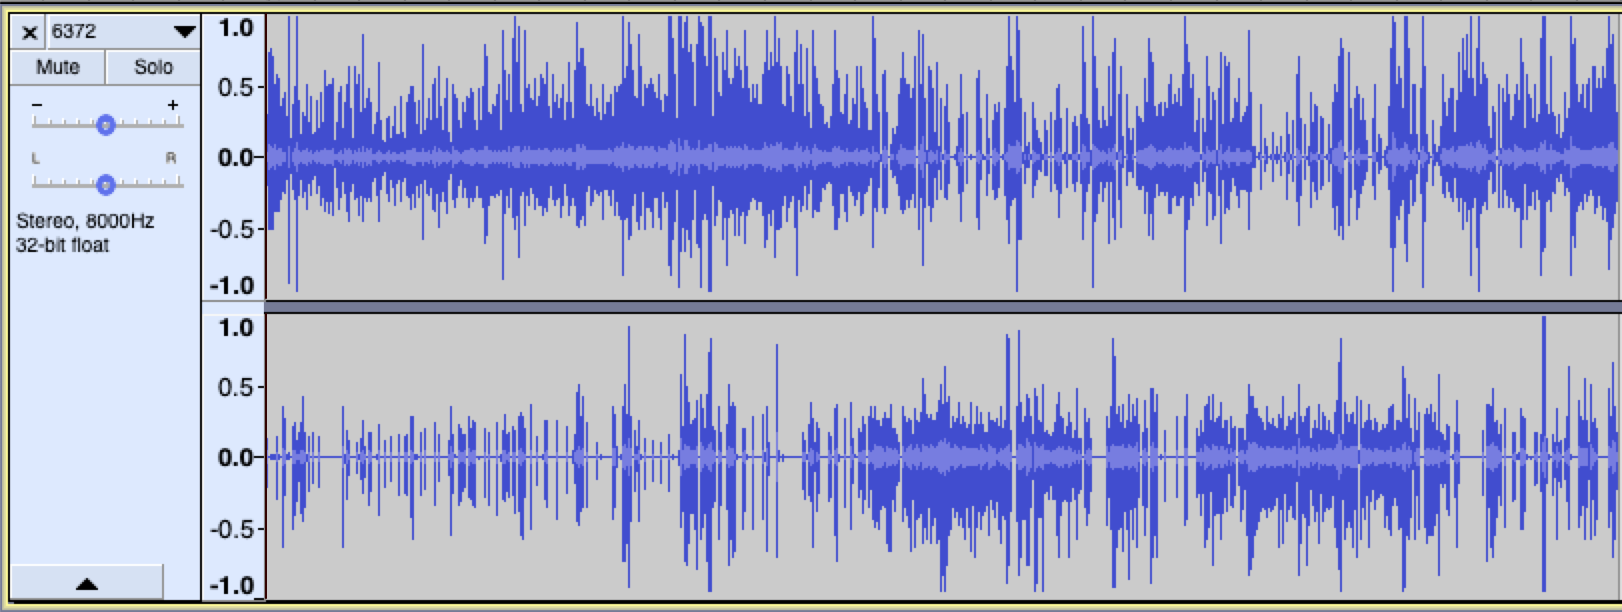
\includegraphics[scale=0.5]{src/main-matter/theory/fig/soundwave_6732_short}
	\caption{Waveform Example. For any conversation audio file a waveform will be read in and digitised through the Calpy software.}
	\label{fig:example_waveform}
%\end{figure}
%
%
%\begin{figure}[h]
	\center
	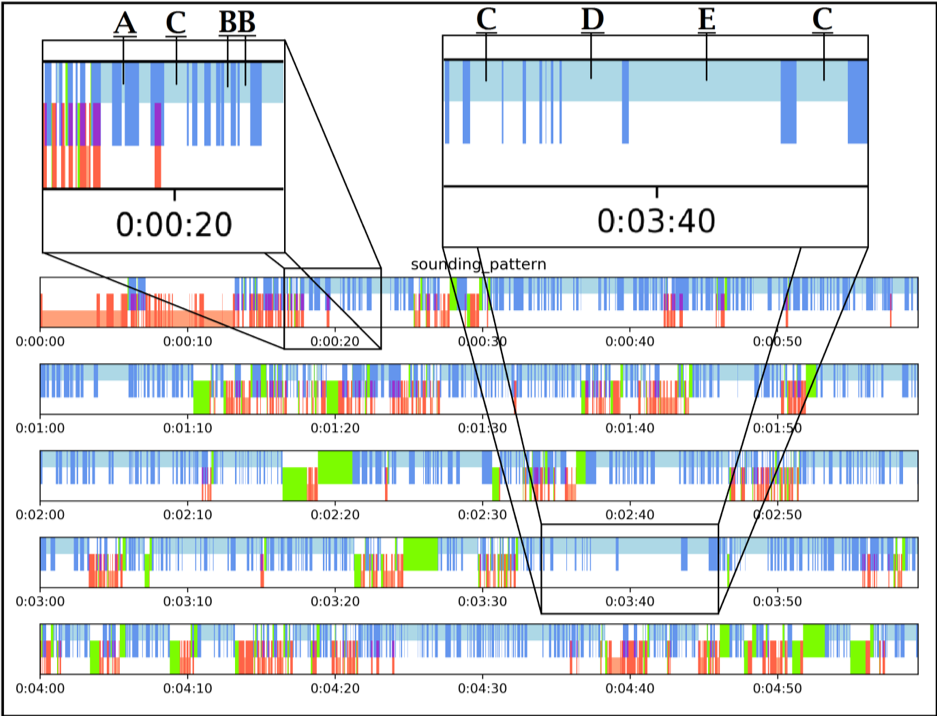
\includegraphics[scale=0.7]{src/main-matter/theory/fig/picture2}
	\caption{Pause code example, a visual representation of the utterances and pauses in an audio file. The light blue and light red both indicate an inner pause (i.e. a pauses bookended by the same speaker), whereas the darker colour indicates utterance. Green represents joint pause (i.e. a pause bookended by different speakers)}
	\label{fig:example_pause-code-symbol}
%\end{figure}
%
%\begin{figure}[h]
	\center
	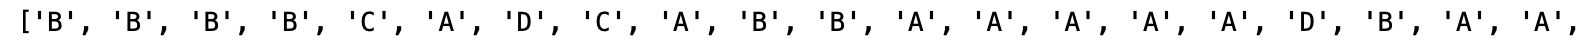
\includegraphics[scale=0.6]{src/main-matter/theory/fig/output_symbols}
	\caption{Symbol Set Example. Each symbol represents a certain pause length defined by the symbol model}
	\label{fig:example_symbol_set}
\end{figure}


\section{Shannon Entropy}
\subsection{Overview}
Shannon Entropy [3] measures the average amount of information delivered through some medium from sender to receiver over a given period of time (or given length of symbols). The idea being new information raises the entropy value, while repeated information lowers it. For this system entropic information must be in a symbolised form such that every occurrence of some defined piece of information can be accurately counted (e.g. pauses).

\subsubsection{Example}
In a telephone conversation there is a level of uncertainty as to what's going to be heard next. The receiver is receiving information from the speaker. Each word delivers some amount of information that can be assigned a value where the value is a measure of how novel the information is that's being presented. If the receiver were to pick words out randomly from the dictionary, it would be almost impossible to predict the next word uttered by the speaker. Thus the entropy would be high for that conversation. Conversely, if the speaker were to say the same word repeatedly, say 'banana', it could be predicted with a high degree of certainty that the next word said is 'banana'. Thus the entropy would tend toward zero for that conversation as there doesn't exist much unpredictability to the information being presented, or another way to say it being there was very little meaningful information being presented.\\

The key aspect of this measure being the symbolisation. This same measure can be applied to anything that can be symbolised (e.g. television, books, radio, etc \ldots), or more specifically looking at the pauses in speech. With that the change in relative proportion of occurrence can be seen so that instances of higher or lower information content than expected can be automatically identified and recorded.


\subsection{Calculating Entropy}
Given a sample set, X, each distinct symbol is written as $x_{i}$, where i is the number of distinct symbols in the symbol set. The entropy model itself is:\\

\centerline{$E(X) = -\sum_i P(x_i)\log P(x_i)$} 

\mediumskip
The value $P(x_i)$ is the probability that a given symbol, $x_i$, occurs in the sample (i.e. its proportion relative to the sample size).

%\subsubsection{Example}
%Sample set = [A, B, A, C, B, C, B, A, B, C, B, A, B, A, C, C, A, B]
%$p(A) = 6/18 = 0.3$

\subsection{Entropy Meaning}
This provides a measure for the randomness vs predictability of the underlying distribution. Having entropy at either bound is unhelpful as it doesn't allow for much inference to be made about the change in meaning. When entropy is at its maximum value no symbol is more likely than any other, thus the symbol probability distribution will be uniform. As soon as one symbol becomes more likely, this decreases the entropy as a level of predictability enters the distribution. \\

When prediction of the next symbol is guaranteed this means no new information is being presented and thus an entropy value of 0 is returned (regardless of symbol model size). The more symbols present in the symbol model the higher the maximum entropy value will be. This doesn't change anything about the way entropy works or what it's representing, it simply allows for a wider distribution of entropy values when more symbols are present such that it will be probabilistically be more unlikely to have a completely non-random system as symbol model size grows. \\ 

\begin{figure}[htbp]
\begin{center}
	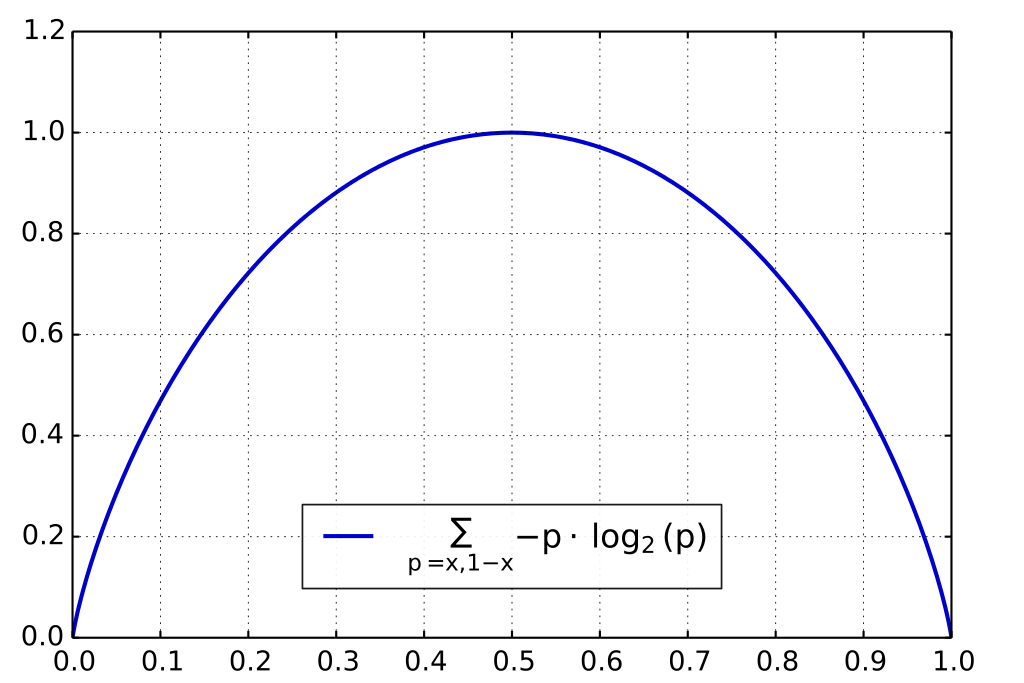
\includegraphics[scale=0.35]{src/main-matter/theory/fig/entropy_model.png}
\caption{Different entropy values for a 2 symbol entropy model across varying symbol probabilities. The point of highest entropy is when both symbols are equally likely at the middle.}
\label{default}
\end{center}
\end{figure}

Figure 2.4 shows the maximum amount of information content for a 2 symbol model being the middle of the entropy model where both symbols are equally likely to occur. From this a ranked probability model can be built ranking the symbols from most likely to least likely to see which symbols are more reliably used for a given conversation. In order for this to work the probability of each symbol must be known. To build this model accurately using entropy means having to wait for every symbol to occur to give those symbols a proper likelihood. 

%This can be interpreted as giving higher entropy values to proportions that  taking the proportion of a given symbols occurrence and giving it a negative weighting from 0 to -infinity where smaller values probabilities receive larger negative weightings that grow exponentially larger negatively. 
%which means \ldots one example being small probabilities carry a big weight because of the log, meaning any low values will decrease the entropy value produced \\
%what else effects the outcome and what else does this tell us about entropy? \\



%
%What is the point of the log2? To put it into binary? Apparently its to maximise low probability outcomes? So if we have something thats super low probability, then the log2 is going to give us a big fat negative number. Whats the purpose of this, it makes low prob important, but what would happen if we didnt have it?\\
%
%\begin{figure}[h]
%	\center
%	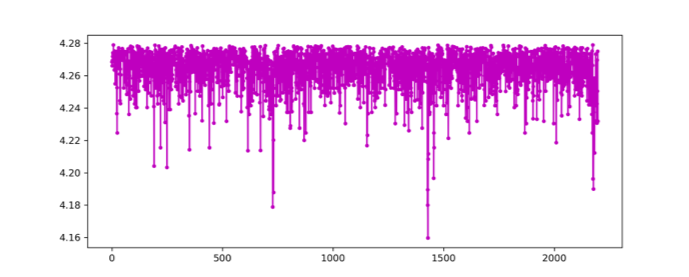
\includegraphics[scale=0.5]{src/main-matter/theory/entropy100}
%	\caption{----}
%	\label{----}
%\end{figure}
%
%\begin{figure}[h]
%	\center
%	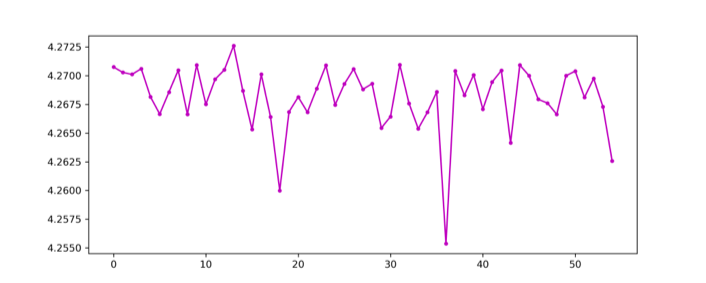
\includegraphics[scale=0.5]{src/main-matter/theory/entropy4000}
%	\caption{----}
%	\label{----}
%\end{figure}




\subsection{Novel Entropy Overview}
The novel entropy method works similarly to how regular entropy works with every symbol given a statistical probability. However, given a symbol set, Shannon entropy will calculate the whole model from scratch. The novel entropy method takes advantage of potentially redundant work by using building a predefined template model, this template can then be referred to quickly to build a new model that only requires a fraction of the sample set compared to classic entropy which requires the entire dataset. If a symbol set were to follow a known distribution (e.g. the ZML law), then regular entropy does redundant work by effectively recomputing the whole model every time it does an entropy calculation as it has to wait for each symbol to occur to give it an accurate probability (based on the sample). Fast entropy instead looks at the proportion of a single given symbol and uses this to extrapolate the rest of the distribution based on the template model provided (i.e. this predefined model represented as the parameters $M, \alpha, \beta, \gamma$). \\

%But this may take quite some time when certain symbols have a naturally low chance of occurring. Instead we can model how our set of symbols should look when ranked from most occurring to least occurring. 

% \begin{figure}
%   \includegraphics[width=\linewidth]{entropy.png}
%   \caption{This appears underbeath.}
%   \label{fig:entropy1}
% \end{figure}

% Figure \ref{fig:boat1} shows a boat. This boat is a metaphor for Entropy. This is below the figure \\
\begin{figure}[h]
	\center
	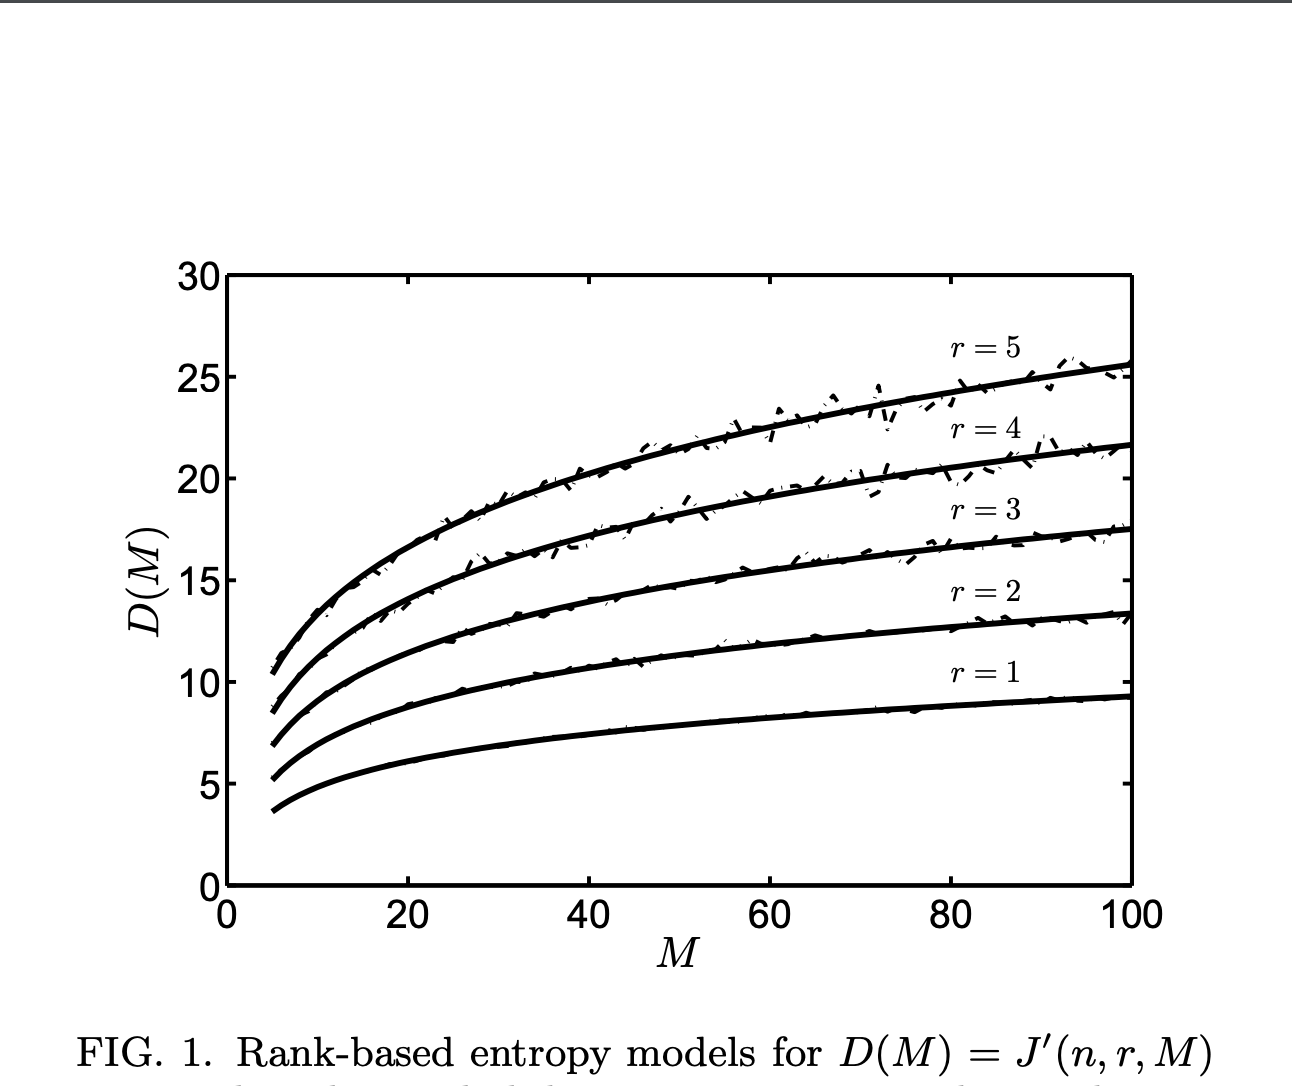
\includegraphics[scale=0.5]{src/main-matter/theory/fig/rank-based-entropy-D(M)}
	\caption{An example of a predefined model following the ZML law used in the novel entropy method [7]}
	\label{----}
\end{figure}
It has been shown in [1] that english letters naturally follow a distribution like the ZML curve (as shown in figure 2.5). This means if pauses can be shown to follow some meaningful distribution like the ZML law then it can be initialised and modelled before new calculations are done such that the system doesn't have to wait for every symbol to occur to measure the total $P(x_i)$ of every symbol, $x_i$. Only the occurrence of a single given symbol, $x_i$, that is expected to occur regularly is needed. With this estimations can be made quickly on samples of the data that have shown to be reliably accurate [7]. \\ 

In this approach windows are used to measure the entropy over a small subset of the sample data, where each window will cover a certain sequential portion of the symbol set. The window size can be increased or decreased to change how the entropy is measured. This is important as too few symbols will not produce meaningful values (e.g. a window of one symbol is meaningless and having only some symbols will be heavily biasing those few symbols), whereas having the whole symbol set as the window will only produce one entropy value (i.e. no change can be inferred from one value). \\

Windows can also overlap other windows to increase the amount of entropy values produced with the same amount of data. For the offline purposes of identifying the information theoretic properties of pause the window overlap is fine. However for an online system too much overlap can make the system extremely slow where the extra computation doesn't produce enough value by receiving diminishing returns on information. \\






